\chapter{Interface générale}
La fenêtre principale de l'application est divisé en cinq parties distinctes comme le montre la figure \ref{fig:ihm}. 

\begin{enumerate}
	\item \textbf{Client}. Vue globale de l'ensemble des clients et des informations qui leurs sont associés
	\item \textbf{Hiérarchie}. Actuellement composé uniquement de la liste des clients
	\item \textbf{Informations détaillées}. Affiche l'ensemble des informations d’un client sélectionné
	\item \textbf{Recherche}. Barre de recherche et filtres associés à la recherche
	\item \textbf{Barre de menu}. Bouton d’actions raccourcis
\end{enumerate}

\begin{figure}[H]
	\centering
	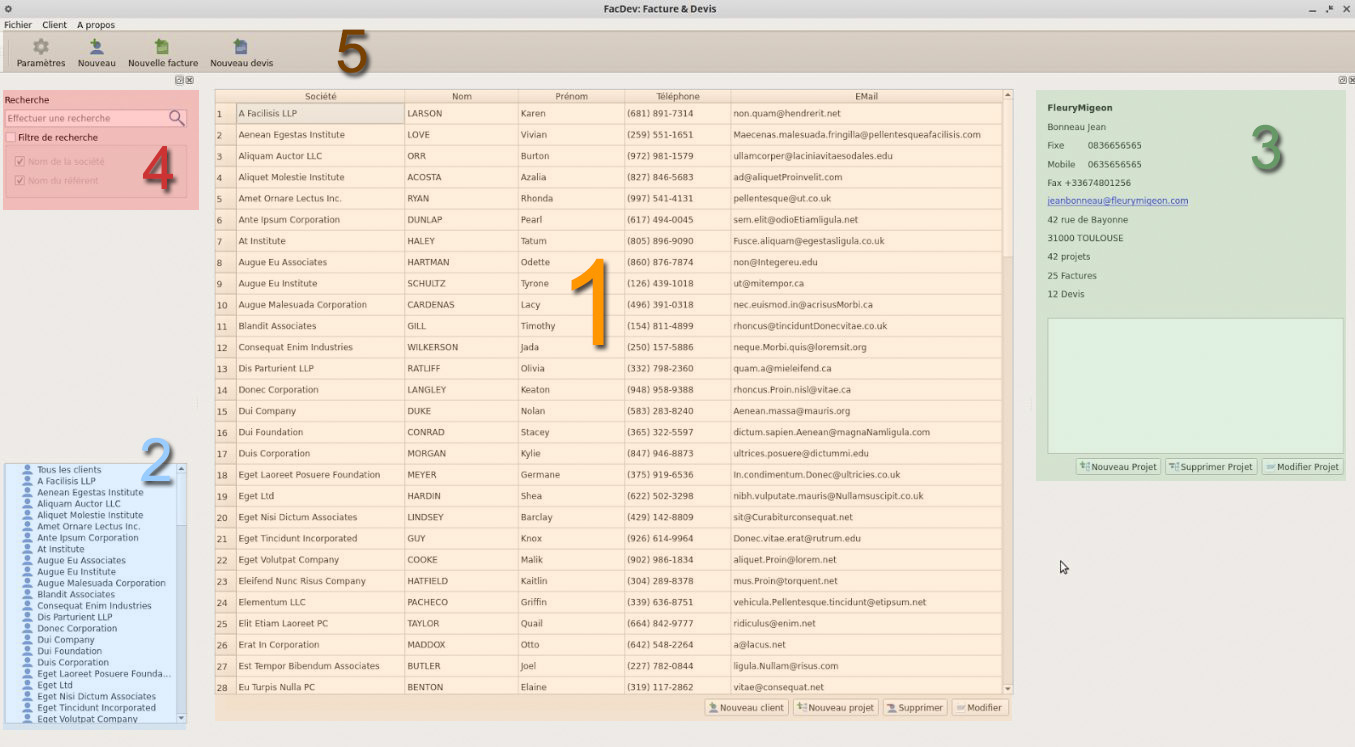
\includegraphics[width=10cm]{screens/ihm.jpg}
	\caption{Interface générale découpée en différentes parties}
	\label{fig:ihm}
\end{figure}

\section{Menus}
La plupart des fonctionnalités du logiciel sont disponibles via les menus situés en haut de l’application. 

\subsection{Fichier}
	\begin{description}
		\item[Paramètres] Permet d'afficher et de d’éditer l’utilisateur du logiciel.
		\item[Quitter] Quitte le logiciel
	\end{description}
\subsection{Client}
\begin{description}
	\item[Nouveau] Ajouter un nouveau client dans la base de données
	\item[Rechercher] Permet de rechercher un client dans la base de données
	\item[Nouvelle facture]  Ajouter une nouvelle facture à un projet d’un client dans la base de données
	\item[Nouveau devis] Ajouter un nouveau devis à un projet d’un client dans la base de données
\end{description}
\subsection{À propos}
\begin{description}
	\item[Qt] Informations sur le framework utilisé
	\item[Fact] Informations sur l'équipe de développement
	\item[FactDev]Informations sur le logiciel
	\item[Icons] Informations sur les icônes utilisées
\end{description}
\section{Barre d'outils}
La barre d’outils permet d’effectuer certaines actions de façon rapide, actions également disponibles via le menu.

\begin{description}
	\item[Paramètres] Permet d'afficher et de d’éditer l'utilisateur du logiciel. Disponible via le menu <<Fichier => Paramètres>>.
	\item[Nouveau] Ajouter un nouveau client dans la base de données. Disponible via le menu <<Client => Nouveau>>.
	\item[Nouvelle facture]  Ajouter une nouvelle facture à un projet d’un client dans la base de données. Disponible via le menu <<Client
		$\rightarrow$
		Nouvelle facture>>
	\item[Nouveau devis] Ajouter un nouveau devis à un projet d’un client dans la base de données. Disponible via le menu <<Client => Nouveau
		devis>>
\end{description}

\section{Panneau du client ou du référent}
Le panneau originellement situé à droite contient les informations du client ou du référent sélectionné, comme le montre la figure
\ref{fig:rightpanel}.

\begin{figure}[H]
	\centering
	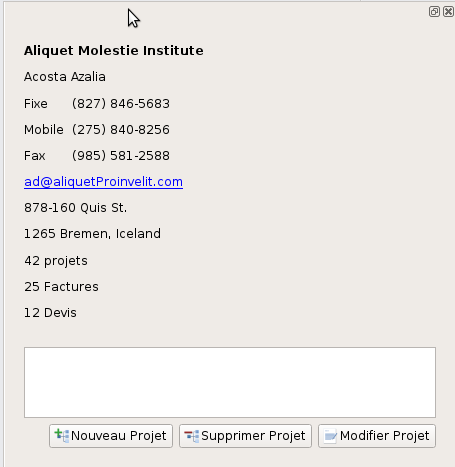
\includegraphics[width=10cm]{screens/dockDroite.png}
	\caption{Panneau du client ou du référent}
	\label{fig:rightpanel}
\end{figure}
% Il est possible d’ajouter un projet, d’en supprimer ou de modifier un projet du client via ce panneau. 
% TODO

\section{Panneau de recherche et sociétés}
Le panneau situé sur la gauche permet d’effectuer une recherche sur le nom de la société ou le nom du client ou du référent si la case
filtre de recherche est cochée et la recherche est faite selon le nom du référent. Cela permet de retrouver rapidement et facilement un
patient.

En dessous du champ de recherche sont affichés toutes les sociétés dans la base de données ainsi que les noms des clients ou référents
lorsque ceux-ci ne possèdent pas de société.




